 \documentclass[letterpaper]{tufte-book}
\usepackage{booktabs}
\usepackage{tabularx}
\usepackage{longtable} 
\usepackage{lscape}
\usepackage{colortbl}
\usepackage{graphicx}
\graphicspath{{../images/}}

\geometry{
  left=.5in,
  right=.5in,
  top=.5in,
  bottom=.5in
}

%\title{Creating a Hierarchical Control Model}

\begin{document}

\begin{landscape}
\advance\vsize0cm
\csname @colroom\endcsname=\vsize
\textheight=\vsize
\csname @colht\endcsname=\vsize

\setlength{\parindent}{0em}
\setlength{\parskip}{.75em}

\begin{multicols}{2}
[ \section{Creating a Hierarchical Control Model}]

\newthought{Definition}

A \textbf{hierarchical control model} is a representation of the system as a combination of control loops depicting the roles and responsibilities of different human and technical components and the relationships (in terms of authority and accountability) that they have to one another.

It consists of:
\begin{compactitem}
\setlength{\itemsep}{0pt}
\setlength{\parskip}{.25em}
\item a \emph{graphical representation} of the relationships components have to one another
%
%Note: in the sense of "nodes and edges" as well as "visual depiction"
\item \emph{annotations} capturing certain information about the system parts depicted
\end{compactitem}

\begin{center}
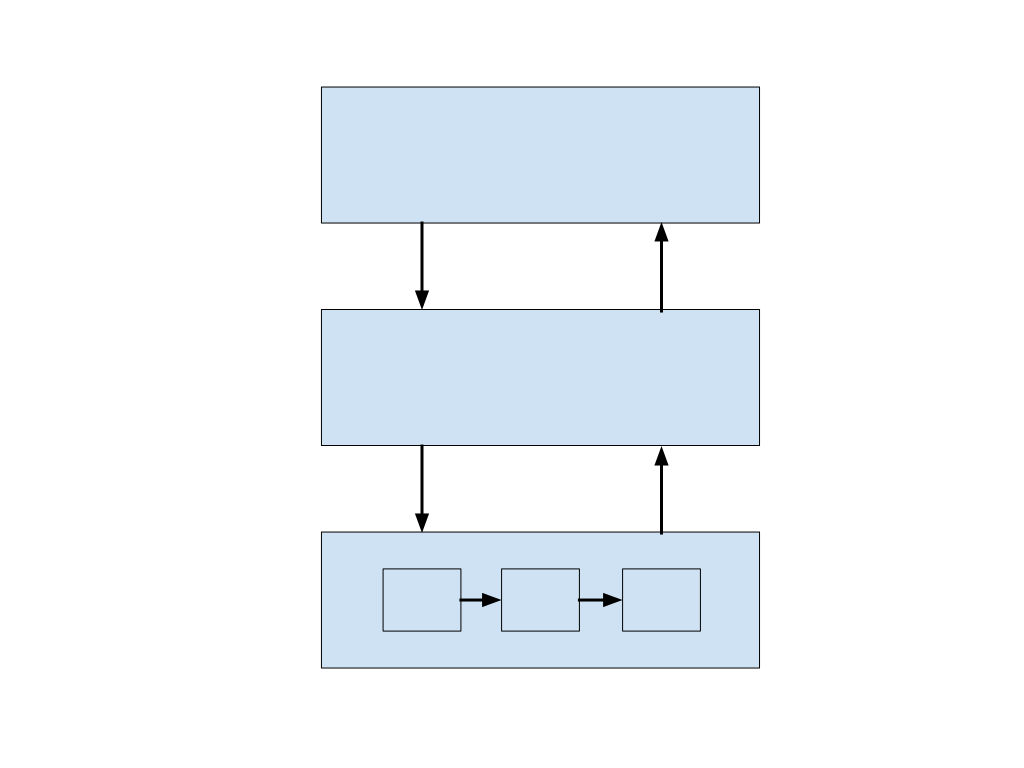
\includegraphics[width=4cm, height=4cm]{generic_model}
\end{center}

\newthought{Visual Conventions}

\begin{compactitem}
 \setlength{\itemsep}{0pt}
\setlength{\parskip}{.25em}
 \item \textsc{boxes}
 
 Each box can represent an abstract process, a human organization or group, an individual human operator, or a technical component.
 \item \textsc{nesting}
 
 Boxes inside others may be used to indicate that the interior elements are sub-processes of the exterior elements.
 \item \textsc{vertical position} 
 
 Items higher on the page exert authority over items lower on the page. 
\item \textsc{arrows} connecting boxes
\begin{compactitem}
		 \setlength{\itemsep}{0pt}
		\setlength{\parskip}{.25em}
		\item down: \emph{control actions} or exerting \emph{authority}
		\item up: \emph{feedback} via sensors, or \emph{accountability}
		\item horizontal: coordination and handoffs between \hbox{processes} or peers.
	\end{compactitem}
 \end{compactitem}
 
 \columnbreak

\textsc{Annotations}
\begin{compactitem}
\setlength{\itemsep}{0pt}
\setlength{\parskip}{.25em}
\item \textsc{goals} 

Specific target outcomes to guide the controlled process towards
\item \textsc{internal process model / mental model}

This includes variables representing the state of the controlled process as perceived by the controller. \emph{Note}: May differ from actual state.
\item \textsc{control algorithm / decision process}

How does the controller choose what actions to take and when?
We do not need to write out the whole algorithm here.
\item \textsc{Available control actions}

We can write a list of the actions and depict them graphically with arrows to the controlled process(es).
We can depict the \emph{actuators} that carry out the actions by noting them along the arrows.
\end{compactitem}

\begin{compactitem}
\item \textsc{Input and instructions} directed to the controller to set goals, etc.
\item \textsc{actuators} to carry out the actions the controller specifies (depicted on arrow edges)
\item \textsc{sensors}

Arrows back from the controlled process to the controller depict \emph{feedback via sensors}, updating the internal process model.
\item \textsc{system being controlled} --- Represented by another box, which may itself be a controller.
\end{compactitem}  

\newthought{Strategic Approaches} 
\begin{compactitem}
\setlength{\itemsep}{0pt}
\setlength{\parskip}{.25em}
\item Start simple, perhaps with only 3 rectangles.
\item Multiple diagrams at different levels of abstraction may be useful.
\end{compactitem}  

\emph{Toolkit}: Hierarchical Control Model Starting Point

\newthought{Relationship to other concepts}

%The \textbf{actions} we list in our model are ones we can analyze to identify \textbf{unsafe control actions}.

When we identify \textbf{causal scenarios} that can lead \textbf{unsafe control actions} to occur, we seek flaws in the control loop the action is part of, using our model to show us what actuators and feedback are relevant.

\pagebreak

\newthought{Thermostat Example}

\begin{itemize}
\setlength{\itemsep}{0pt}
\setlength{\parskip}{.25em}
\item \textbf{Goal}: Adjust the room's temperature to 72 degrees F (TARGET)
\item \textbf{Internal Process Model / Mental Model}: 

Measured room temperature: 69 degrees F; Current heater state: ON
\item \textbf{Control Algorithm / Decision Process}
  \begin{compactitem}[*]
    \setlength{\itemsep}{0pt}
    \setlength{\parskip}{.25em}
  \item If MEASURED $<=$ TARGET $-$ 2: Turn HEAT ON.
  \item If MEASURED $>=$ TARGET $+$ 2 : Turn HEAT OFF.
  \item Else: Do nothing.
  \end{compactitem}
\item \textbf{Control Actions}: Turn heater ON, Turn heater OFF 
\item \textbf{Input} --- A human operator enters the TARGET temperature
\item \textbf{Sensor} --- A thermometer reports the temperature in degrees Farenheit
\item \textbf{Actuator} --- We could consider the furnace and heaters an actuator the thermostat uses to adjust the temperature of the apartment's air, or there is an actuator that switches the furnace on or off when signalled by the thermostat.
\item \textbf{System being controlled} --- The thermostat is controlling the heater directly and the temperature of the apartment indirectly.
\end{itemize}  









Note: The ACTUAL temperature may differ from MEASURED (e.g. ACTUAL might be 68 degrees F while MEASURED is 69 degrees F).

 \columnbreak
 
 \newthought{Thermostat Diagram}

\begin{center}
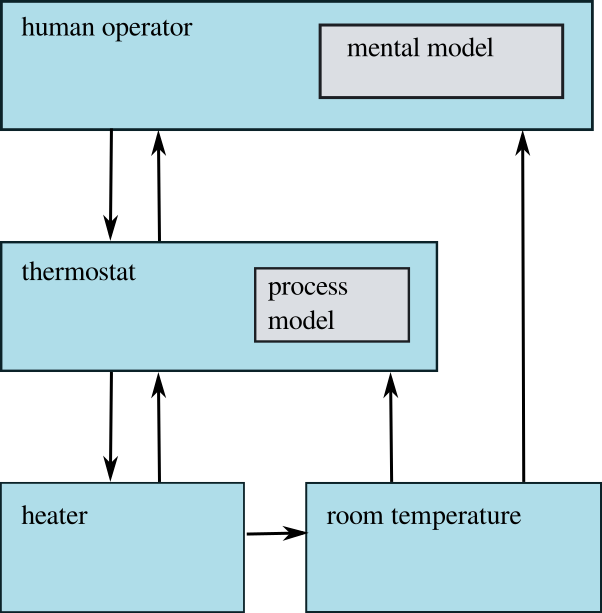
\includegraphics[width=8cm]{thermostat_model}
\end{center}
 
\end{multicols}
\end{landscape}
\end{document}
